\documentclass[conference,10pt,letterpaper]{IEEEtran}
\IEEEoverridecommandlockouts
\usepackage[T1]{fontenc}
\usepackage[utf8]{inputenc}
\usepackage{mathptmx}          % Times text and math
\usepackage{amsmath}
\usepackage{graphicx}
\usepackage{array}
\usepackage{booktabs}
\usepackage{cite}             % IEEE citation lists: [3], [5] and ranges [3]--[5]
\usepackage{xurl}
\usepackage[hidelinks]{hyperref}
\graphicspath{{figures/}}
\raggedbottom
\begin{document}
\bstctlcite{IEEEexample:BSTcontrol}   % et al. after six authors, no dash for repeated authors (see references.bib)

\title{BERT-Based Requirement Classification for Agile Backlog Management}
\author{\IEEEauthorblockN{Gaurav Rajbhar}\IEEEauthorblockA{School of Computer Science and Engineering\\{}Lovely Professional University\\{}Phagwara, Punjab, India\\{}gauravrajbhar2115@gmail.com}}
\maketitle
\begin{abstract}Product backlogs mix feature requests, quality constraints, defects and chores, and few teams label them consistently, so quality requirements tend to surface late, when they are costly to fix. This paper asks whether BERT-family encoders can classify backlog items reliably enough to support refinement. We synthesise 35 sources and propose a two-level framework whose calibrated confidence gate sends uncertain items to the Product Owner. On PROMISE NFR (625 requirements, 15 projects) we fully fine-tuned DistilBERT, BERT and RoBERTa and compared them with a TF-IDF support vector machine (SVM) under random and project-held-out splits over three seeds; models trained on all of PROMISE were then tested on 327 industrial requirements from four other projects. On random folds all models tied on functional versus non-functional classification (macro-F1 0.909–0.917). On unseen projects every score fell, but the transformers fell less (0.736–0.806 versus 0.590 for the SVM; project-bootstrap intervals excluded zero in eight of nine runs). On the industrial requirements they led the SVM by 0.070–0.081 macro-F1, but confidence thresholds set on PROMISE met their precision target in only 5 of 8 runs. We conclude that BERT classifiers suit refinement assistance better than autonomous labelling.\end{abstract}
\begin{IEEEkeywords}requirements classification, BERT, RoBERTa, non-functional requirements, cross-project evaluation, calibration, agile, product backlog, PROMISE NFR\end{IEEEkeywords}

\section{Introduction}\label{sec:intro}
In Scrum the Product Backlog is the single, ordered source of work for a team, and the Product Owner is accountable for keeping it in order~\cite{scrumguide2020}. In practice the backlog is messier than that one sentence suggests. In a grounded-theory study of eight projects and 56 interviews at Pivotal, Sedano et al.~\cite{sedano2019} found that the backlog acts as an informal model of the work still to be done, and that it serves as a boundary object shared by the different roles on a team rather than as a requirements specification. User stories are an increasingly popular way to write these items; Lucassen et al.~\cite{lucassen2016use} surveyed 182 practitioners and interviewed 21 more, and found the Connextra template (“As a $\langle$role$\rangle$, I want $\langle$goal$\rangle$, so that $\langle$benefit$\rangle$”) to be the dominant format.

Consider a typical story: “As a user, I want to reset my password through an e-mailed link so that I can regain access to my account.” On the surface it is functional. Read carefully, it also carries security obligations: the link must expire, it must work only once, and the response must not reveal whether an e-mail address is registered. If the team tags the story only as a feature, those constraints are easily missed until a penetration test or an incident exposes them. Dalpiaz et al.~\cite{dalpiaz2019} formalised this observation by annotating requirements with separate functional and quality \emph{aspects}, so that a single item can carry both. Van Can and Dalpiaz~\cite{vancan2025} analysed 1,636 backlog items from 14 projects and found that requirement-related content is labelled inconsistently and that one item often contains several requirements at different levels of granularity.

Automatic classification of requirements text has a long history. It started with indicator-term classifiers trained on student specifications~\cite{clelandhuang2007} and moved through feature-engineered support vector machines~\cite{kurtanovic2017,diascanedo2020} and convolutional or recurrent networks~\cite{rahman2019,rahimi2021}. Since BERT appeared~\cite{devlin2019}, fine-tuned transformers have become the default, and NoRBERT showed that transfer learning helps most on projects not seen during training~\cite{hey2020norbert,hey2022corrected}. Yet three gaps remain. First, most results on FR/NFR classification come from the PROMISE NFR corpus~\cite{promisenfr2007}, 625 “shall” statements written for 15 student projects in the mid-2000s, or from its extensions, not from agile backlogs. Second, scores are reported under very different protocols, so a 0.99 in one paper and a 0.87 in another cannot be compared directly. Third, few of the studies we reviewed say what a team should \emph{do} with a predicted label, or how to handle the predictions a model is unsure about.

This paper addresses those gaps with four contributions:

\begin{enumerate}
\item a critical synthesis of 35 sources, with the reported results collected in a single comparison table (Table~\ref{tab:lit}) that keeps each study's dataset and protocol visible;
\item a two-level classification framework (Figs. \ref{fig:arch}–\ref{fig:flow}) that connects predicted labels to backlog refinement, the Definition of Done and sprint planning, and that routes uncertain items to a human through an explicit confidence gate;
\item a comparative experiment that we ran ourselves: fully fine-tuned DistilBERT, BERT and RoBERTa against a TF-IDF SVM on PROMISE NFR, on identical random and project-held-out folds over three seeds, followed by a test on industrial requirements from four other projects and an analysis of calibration, with every setting stated and saved predictions from which every number can be recomputed;
\item a discussion of deployment challenges and threats to validity, summarised in Table~\ref{tab:chal}.
\end{enumerate}

Section~\ref{sec:rw} reviews related work, Section~\ref{sec:method} presents the framework, Section~\ref{sec:exp} reports our experiments and the literature results separately, Section~\ref{sec:disc} discusses challenges and validity, and Section~\ref{sec:concl} concludes.

\section{Related Work}\label{sec:rw}
\begin{figure*}[!t]
\centering
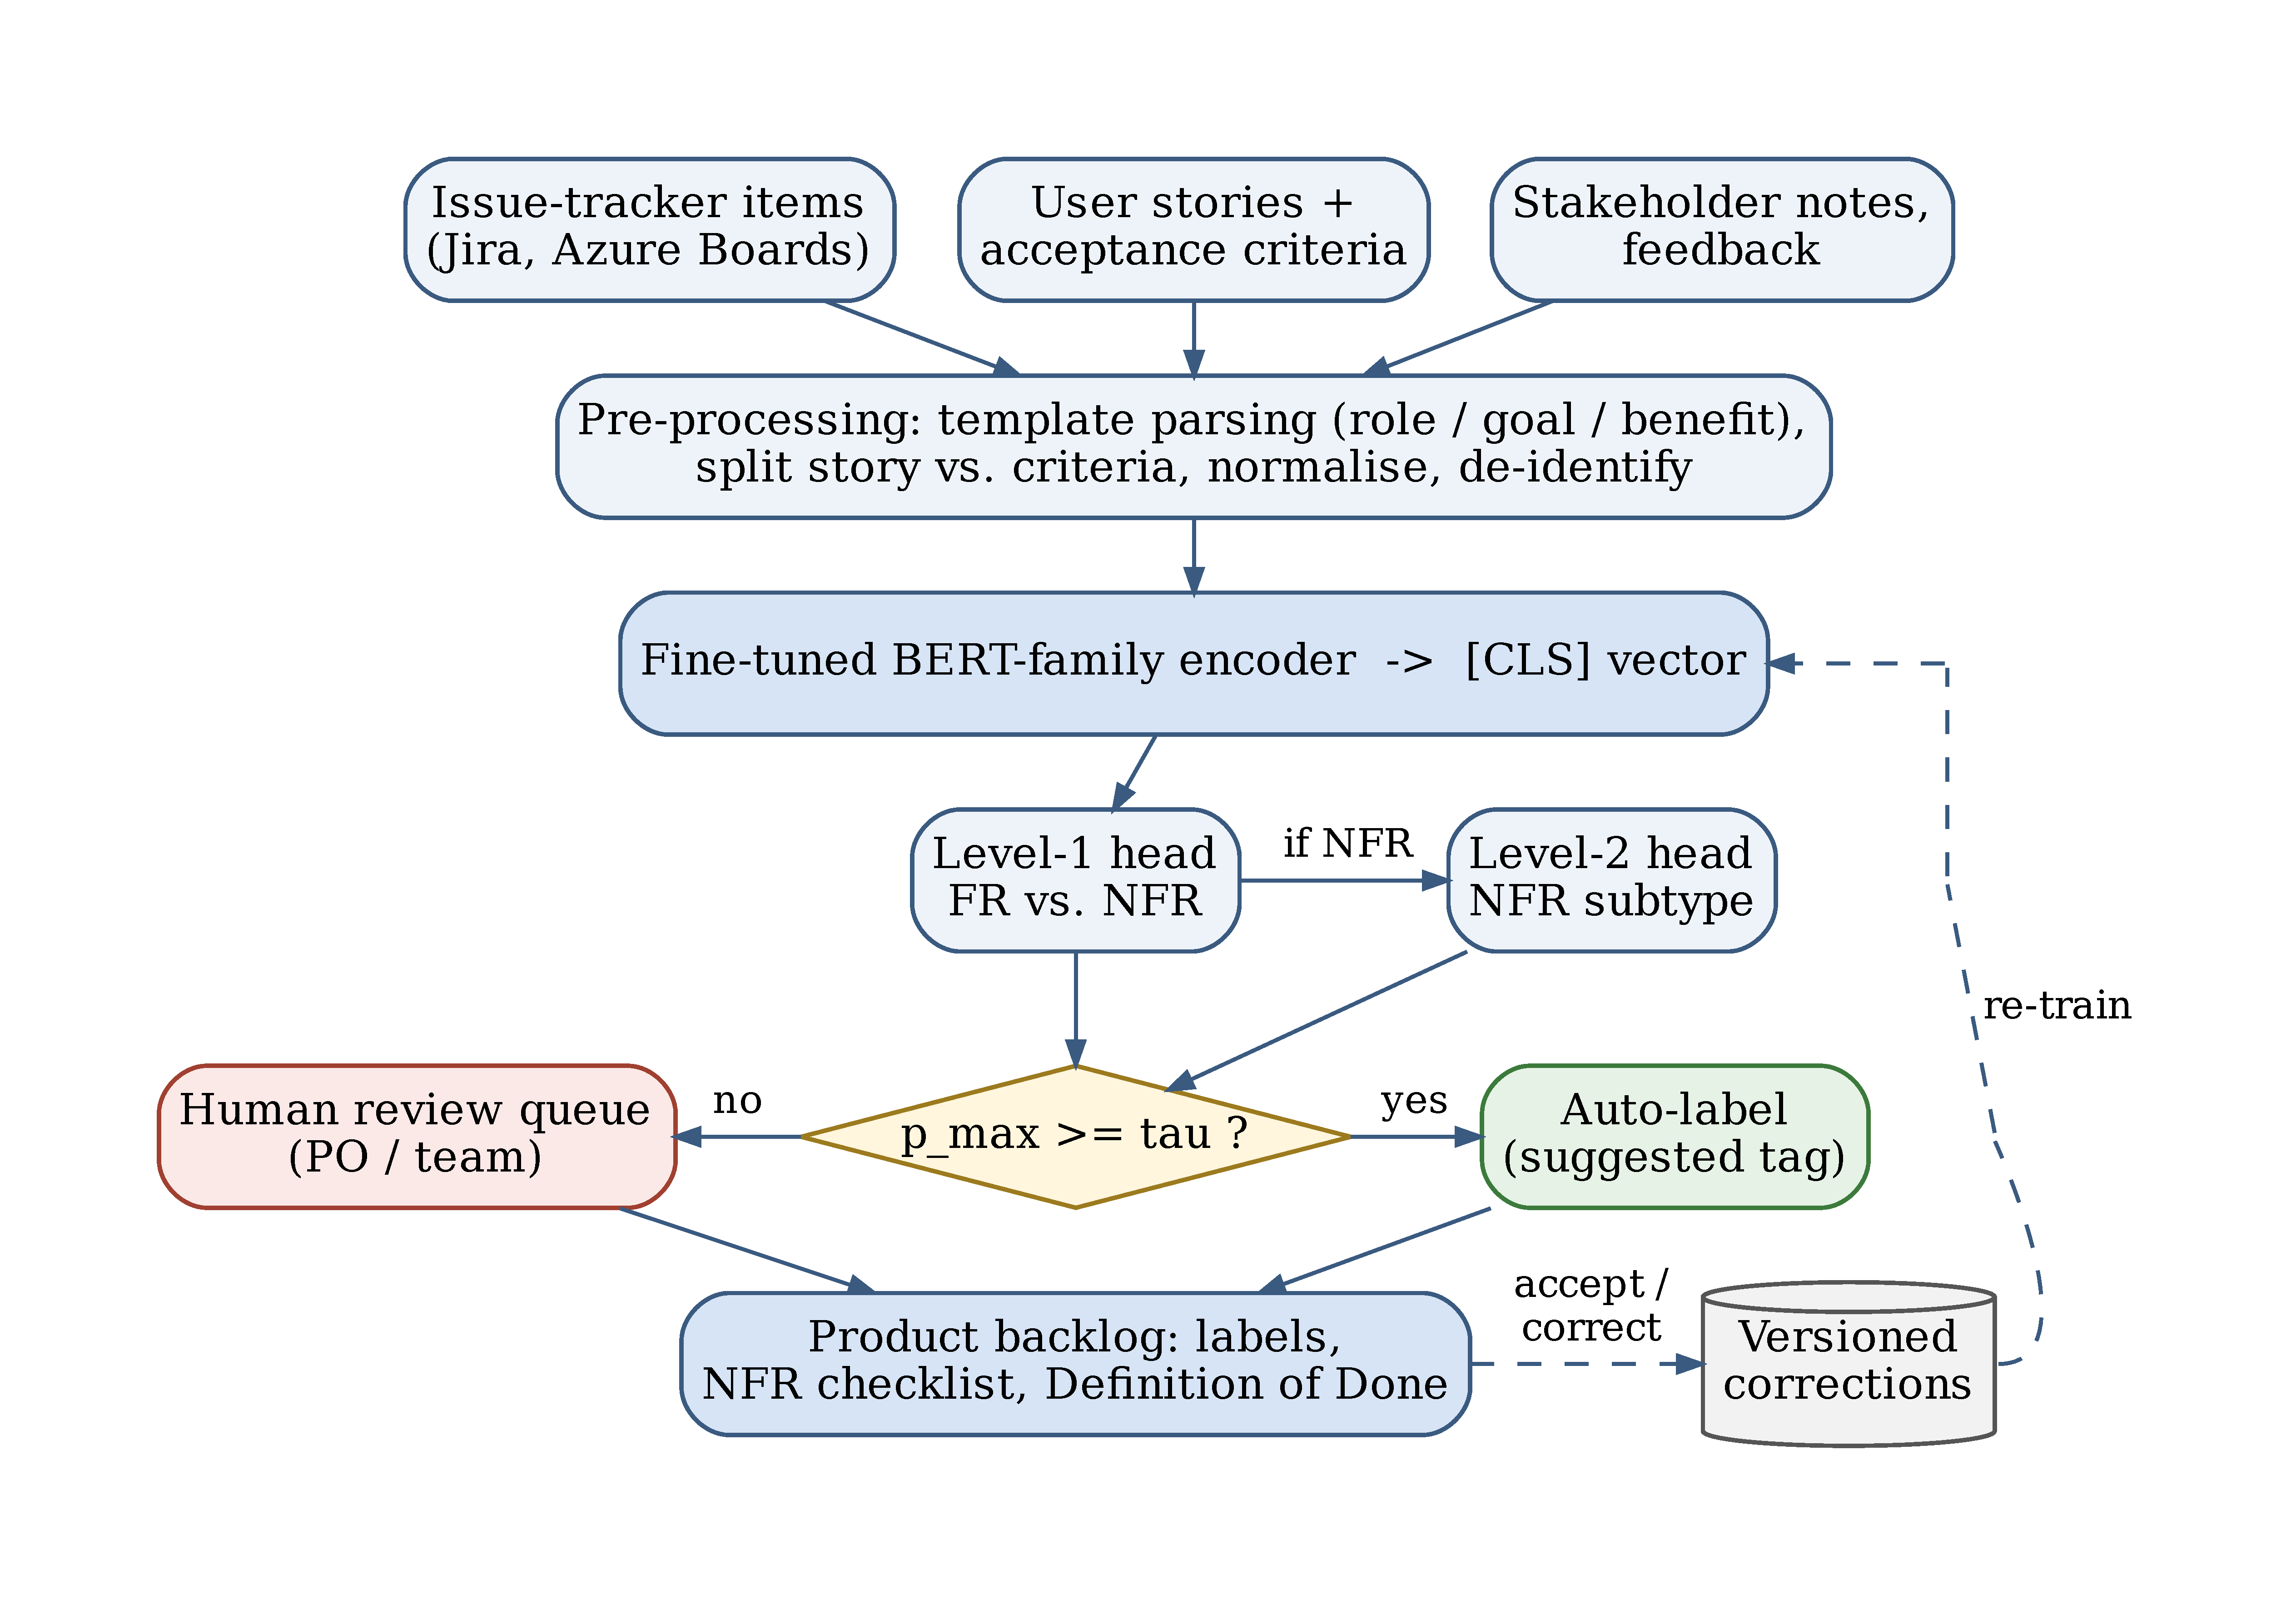
\includegraphics[width=0.94\textwidth]{fig1_architecture.pdf}
\caption{Proposed framework. Items are normalised, encoded by a fine-tuned BERT-family model and classified at two levels. A confidence gate decides whether a label is applied automatically or sent to the Product Owner, whose corrections feed periodic re-training.}
\label{fig:arch}
\end{figure*}

\subsection{Datasets and Label Schemes}
The PROMISE NFR dataset was created by Cleland-Huang et al.~\cite{clelandhuang2007} and later shared through the PROMISE repository~\cite{promisenfr2007}. It contains 255 functional requirements and 370 non-functional ones, the latter spread over eleven quality classes ranging from usability (67 items) to portability (one item). Lima et al.~\cite{lima2019} enlarged it to 969 requirements (444 functional, 525 non-functional) in PROMISE\_exp, but kept the same style of text. Dalpiaz et al.~\cite{dalpiaz2019} relabelled more than 1,500 requirements from PROMISE and seven industrial documents with independent functional and quality aspects. That relabelling is important because it shows that the binary FR/NFR split, which most papers take for granted, forces an annotator to discard information whenever a requirement constrains behaviour and quality at the same time.

\subsection{Classical and Deep-Learning Classifiers}
Kurtanović and Maalej~\cite{kurtanovic2017} combined lexical and syntactic features with a support vector machine and used under- and over-sampling to counter class imbalance. They reported precision and recall of up to about 92\% for the FR/NFR distinction on PROMISE NFR, with security and performance among the best-recognised quality classes. Dalpiaz et al.~\cite{dalpiaz2019} replaced the large feature space with 17 interpretable features derived from dependency parsing. Their classifier fitted the training data slightly less well than a reconstruction of the Kurtanović and Maalej model, but it generalised better to other datasets and its decisions could be explained. To us this is the more useful result for practice, because a Product Owner is more likely to trust a tag whose cause can be shown. Dias Canedo and Cordeiro Mendes~\cite{diascanedo2020} compared bag-of-words, TF-IDF and chi-squared features with logistic regression, SVM, multinomial Naive Bayes and k-nearest neighbours on PROMISE\_exp. TF-IDF with logistic regression gave the best F-measure: 0.91 for FR/NFR (tied with the SVM), 0.74 for the NFR classes and 0.78 overall. These are the same feature and model families as our baselines in Section~\ref{sec:exp}.

Subsequent studies moved to neural architectures. Rahman et al.~\cite{rahman2019} compared recurrent variants on PROMISE NFR and reported that an LSTM reached a validation precision of 0.973, recall of 0.967 and F1 of 0.966, ahead of GRU and CNN models. Rahimi et al.~\cite{rahimi2021} combined LSTM, BiLSTM, GRU and CNN models in an ensemble on a 17-class PROMISE variant that also labels functional subtypes, and reported 92.56\% accuracy for one-phase classification. Their two-phase variant reached 95.7\% for the binary step and 93.4\% for the multi-class step. Two reviews put this stream in context: Binkhonain and Zhao~\cite{binkhonain2019} catalogued machine-learning methods for identifying non-functional requirements, and Zhao et al.~\cite{zhao2022nlp4re} mapped the wider NLP-for-RE field and documented the gap between research prototypes and tools that practitioners actually use.

A pattern runs through several of these numbers, although not all of them. Some of the highest scores come from small evaluation sets, from validation rather than test data, or from briefly described splits. The F1 of 0.966 reported by Rahman et al.~\cite{rahman2019} is an average over cross-validation folds of PROMISE NFR's roughly 370 non-functional requirements; on a separately selected test set, the same LSTM averaged an F1 of 0.70. Under random cross-validation, requirements from the same project, often with near-identical wording, fall on both sides of a split. Not every high score fits this pattern, however: Eltahier et al.~\cite{eltahier2025} also report 0.97 on a second dataset, FR\_NFR. A high random-fold score says little about how the same model would label a new team's backlog.

\subsection{BERT and Its Variants in Requirements Engineering}
BERT pre-trains a bidirectional transformer encoder with masked-language-model and next-sentence objectives, and is then adapted to a downstream task by adding a single output layer and fine-tuning all weights~\cite{devlin2019}. RoBERTa keeps the architecture but trains longer on more data, drops the next-sentence objective and masks tokens dynamically~\cite{liu2019roberta}. Sanh et al.~\cite{sanh2019distilbert} compressed BERT into DistilBERT by knowledge distillation and reported that the student model has 40\% fewer parameters, runs inference 60\% faster and retains 97\% of BERT's performance on the GLUE language-understanding benchmark, which makes it a realistic choice for a team without GPUs.

NoRBERT was an early and widely cited application of BERT fine-tuning to requirements classification~\cite{hey2020norbert}. On PROMISE NFR it reached an F1 of up to 94\% for FR/NFR and an average F1 of 87\% on the most frequent quality classes. In an unseen-project setup on a relabelled version of PROMISE it reported an improvement of 15 percentage points over earlier approaches. The authors later released a corrected version, citing a bug in part of the evaluation, in which that improvement is ten percentage points~\cite{hey2022corrected}. We regard this correction as one of the most instructive episodes in the field. It shows how much the split protocol can change a headline number, and it was disclosed openly.

Subsequent studies applied transformer encoders across a wider range of corpora. Kici et al.~\cite{kici2021} found that DistilBERT outperformed LSTM and BiLSTM baselines on several requirements datasets. Luo et al.~\cite{luo2022prcbert} reformulated classification as prompt-based cloze filling (PRCBERT). A model fine-tuned on PROMISE and transferred without labels, with self-learning, reached weighted F1 scores of 53.27\% on NFR-Review and 72.96\% on NFR-SO. Domain-specific work includes aeroBERT, fine-tuned on a corpus of 310 aerospace requirements, which reached an average F1 of 0.83 on a 31-item test set~\cite{tikayatray2023}. Alsanoosy~\cite{alsanoosy2026} assembled 4,908 requirements and reported a binary F1 of 86.93\% for a BERT+LSTM hybrid, while Eltahier et al.~\cite{eltahier2025} reported an average F1 of 0.99 on PROMISE and 0.97 on the FR\_NFR dataset. Their protocol is stratified 10-fold cross-validation with weighted F1, and hyper-parameters were chosen by ablation on the same data. Read side by side, these results show that the dataset and the split protocol explain more of the variation than the choice of encoder. A score of 0.99 on PROMISE and 0.87 on a corpus eight times larger do not show that one method is better than the other.

\subsection{Zero-Shot, Few-Shot and Large Language Models}
Labelling is expensive, so learning from few or no labelled examples is attractive. Alhoshan et al.~\cite{alhoshan2023} tested zero-shot classification with pre-trained sentence embeddings and label descriptions. Their best zero-shot F1 was 0.66 for functional and 0.65 for non-functional requirements, against supervised F1 scores of 0.93 for the Kurtanović–Maalej SVM on FR and 0.93 for NoRBERT on NFR, which they took from the original studies. The gap is large but so is the saving: no labelled data at all. SetFit contrastively fine-tunes a sentence transformer on pairs of labelled examples; with eight labelled examples per class on the Customer Reviews sentiment dataset it was competitive with RoBERTa-Large fine-tuned on the full training set~\cite{tunstall2022setfit}. Petrillo et al.~\cite{petrillo2025} applied SetFit and fine-tuned transformers to security-requirements classification on the SecReq dataset. We did not find a study that applies SetFit to PROMISE NFR, although our search was not systematic. The broader shift towards large language models is documented in the review by Hou et al.~\cite{hou2024llm4se}. For backlogs specifically, van Can and Dalpiaz~\cite{vancan2025} found that fine-tuned encoder-only models were better suited than prompted generative models to locating requirements in backlog items. This is a useful corrective to the assumption that the largest model is always the right one.

\subsection{Agile Backlog Support}
Other work automates neighbouring backlog tasks. Lucassen et al.~\cite{lucassen2016qus} proposed the Quality User Story framework, with 13 criteria, and the AQUSA tool for detecting defects in story text. Mejía-Domínguez et al.~\cite{mejia2026loona} built LOONA for the quality assurance of Spanish user stories: a fine-tuned Spanish BERT classifier flags defective stories, and a confidence threshold decides when a generative model proposes a rewrite. The classifier reached an F1 of 0.91 in 5-fold cross-validation on expert-labelled stories. Prioritisation is the step that ultimately consumes any label, and Hujainah et al.~\cite{hujainah2018} reviewed the techniques, stakeholders and open challenges of requirements prioritisation. None of the studies cited in this subsection feeds requirement-type labels into prioritisation or refinement, and that is the link our framework is meant to provide.

\begin{table*}[!t]
\centering
\caption{Reported results from the literature (not our experiments). Scores are copied as published; datasets and protocols differ, so rows are not directly comparable.}
\label{tab:lit}
\footnotesize
\setlength{\tabcolsep}{3pt}
\renewcommand{\arraystretch}{1.12}
\begin{tabular}{>{\raggedright\arraybackslash}p{2.3cm}>{\raggedright\arraybackslash}p{3.0cm}>{\raggedright\arraybackslash}p{3.1cm}>{\raggedright\arraybackslash}p{4.3cm}>{\raggedright\arraybackslash}p{3.6cm}}
\toprule
\textbf{Study} & \textbf{Data} & \textbf{Approach} & \textbf{Result as reported by the authors} & \textbf{Our remark} \\
\midrule
\cite{kurtanovic2017} & PROMISE NFR & SVM, lexical + syntactic features, sampling & FR/NFR P and R up to $\approx$92\% & Strong classical baseline \\
\cite{dalpiaz2019} & PROMISE + 7 industrial sets (\textgreater{}1,500 items), F/Q aspects & Dependency-parse features (17) & Generalises better than K\&M reconstruction & Interpretable; multi-aspect labels \\
\cite{diascanedo2020} & PROMISE\_exp (969) & TF-IDF / BoW / CHI2 + LR, SVM, MNB, kNN & TF-IDF+LR F 0.91 (FR/NFR, tie with SVM); 0.74 (NFR classes) & Same model families as our baselines \\
\cite{rahman2019} & PROMISE NFR & LSTM / GRU / CNN & LSTM (validation): P 0.973, R 0.967, F1 0.966 & Test-set F1 0.70 \\
\cite{rahimi2021} & PROMISE, 17-class variant & Ensemble of DL models & Acc. 95.7\% (binary), 93.4\% (multi-class), two-phase & Accuracy only \\
\cite{hey2020norbert} & PROMISE NFR & NoRBERT (BERT fine-tuning) & FR/NFR F1 up to 94\%; frequent NFR avg. F1 87\% & Unseen-project gain 15 pp, corrected to 10 pp~\cite{hey2022corrected} \\
\cite{kici2021} & PROMISE NFR and others & DistilBERT & Outperformed LSTM and BiLSTM & Light model \\
\cite{luo2022prcbert} & NFR-Review, NFR-SO & PRCBERT prompt learning & Transferred, no labels: weighted F1 53.27\% / 72.96\% & Non-SRS text \\
\cite{alhoshan2023} & PROMISE NFR and others & Zero-shot embeddings & Best F1 0.66 (FR), 0.65 (NFR) & No labels needed \\
\cite{tikayatray2023} & 310 aerospace requirements & aeroBERT-Classifier & Average F1 0.83 & 31-item test set \\
\cite{petrillo2025} & SecReq (623, 3 specifications) & Fine-tuned transformers; SetFit & Best few-shot (SetFit, BERT body, augmented data): Acc. 0.94, F1 0.90 & Security vs. other only \\
\cite{alsanoosy2026} & 4,908 requirements & BERT + LSTM & Binary F1 86.93\% & Largest corpus here \\
\cite{eltahier2025} & PROMISE; FR\_NFR & BERT fine-tuning variants & Weighted F1 0.99 (PROMISE), 0.97 (FR\_NFR) & Tuned on the evaluation data \\
\cite{vancan2025} & 1,636 backlog items, 14 projects & Encoders vs. generative LLMs & Encoder-only models most suitable & Closest to backlogs \\
\bottomrule
\end{tabular}
\end{table*}

\section{Methodology and Proposed Framework}\label{sec:method}
\subsection{Research Approach}
The study combines a structured, but not systematic, literature review with our own experiments. In October 2026 we gathered candidate papers published across IEEE Xplore, the ACM Digital Library, SpringerLink, ScienceDirect, MDPI and arXiv using keyword queries of \emph{requirements classification}, \emph{non-functional}, \emph{BERT}, \emph{user story}, \emph{product backlog}, \emph{zero-shot} and \emph{class imbalance}. We screened the candidate records and kept 35. A source was kept if it reported a classifier for natural-language requirements, contributed a dataset or model that such work depends on, or described agile backlog practice. Every DOI and its bibliographic record were verified against the public registry record before inclusion. Because we did not follow a registered protocol, did not double-screen, and did not snowball exhaustively, we do not claim the coverage of a systematic literature review.

\subsection{Framework Overview}
Fig.~\ref{fig:arch} shows the proposed framework. Items enter from the team's tracker (for example Jira), from a story-writing workshop or from user feedback. A pre-processing step normalises each item: it splits a Connextra story into role, goal and benefit, keeps the “so that” clause because it often signals the quality concern, separates acceptance criteria, and removes personal names. Classification then proceeds in two levels. Level 1 decides whether an item contains a quality concern: FR versus NFR, or F+Q when both aspects are present, as proposed by Dalpiaz et al.~\cite{dalpiaz2019}. Level 2 assigns the quality class, such as security (SE), performance (PE), usability (US) or operability (O), and is run only for items that Level 1 flags.

\subsection{Encoder and Training Objective}
Any BERT-family encoder fits the framework; in Section~\ref{sec:exp} we compare DistilBERT, BERT-base and RoBERTa-base. Fig.~\ref{fig:ft} traces the running example through the model. The text is split into subword units (WordPiece for BERT and DistilBERT, byte-level byte-pair encoding for RoBERTa), the final hidden state of the first token passes through a small classification head, and a softmax gives a probability for each of the $K$ labels. PROMISE NFR is imbalanced: usability has 67 examples and fault tolerance has 10. The training loss therefore weights each class by its inverse frequency, a common algorithm-level remedy for imbalance that is implemented through a weight or cost scheme~\cite{johnson2019}:

\begin{equation}
\mathcal{L} = -\frac{1}{N}\sum_{i=1}^{N} w_{y_i}\,\log p_\theta(y_i \mid x_i), \qquad w_c = \frac{N}{K\,N_c}
\label{eq:wce}
\end{equation}
Here $N$ is the number of training items, $N_c$ the number of items in class $c$ and $K$ the number of classes. Re-sampling, as used by Kurtanović and Maalej~\cite{kurtanovic2017}, is an alternative. We prefer weighting because it leaves the data untouched and adds no duplicated sentences that could appear in both training and test folds.

\begin{figure}[!t]
\centering
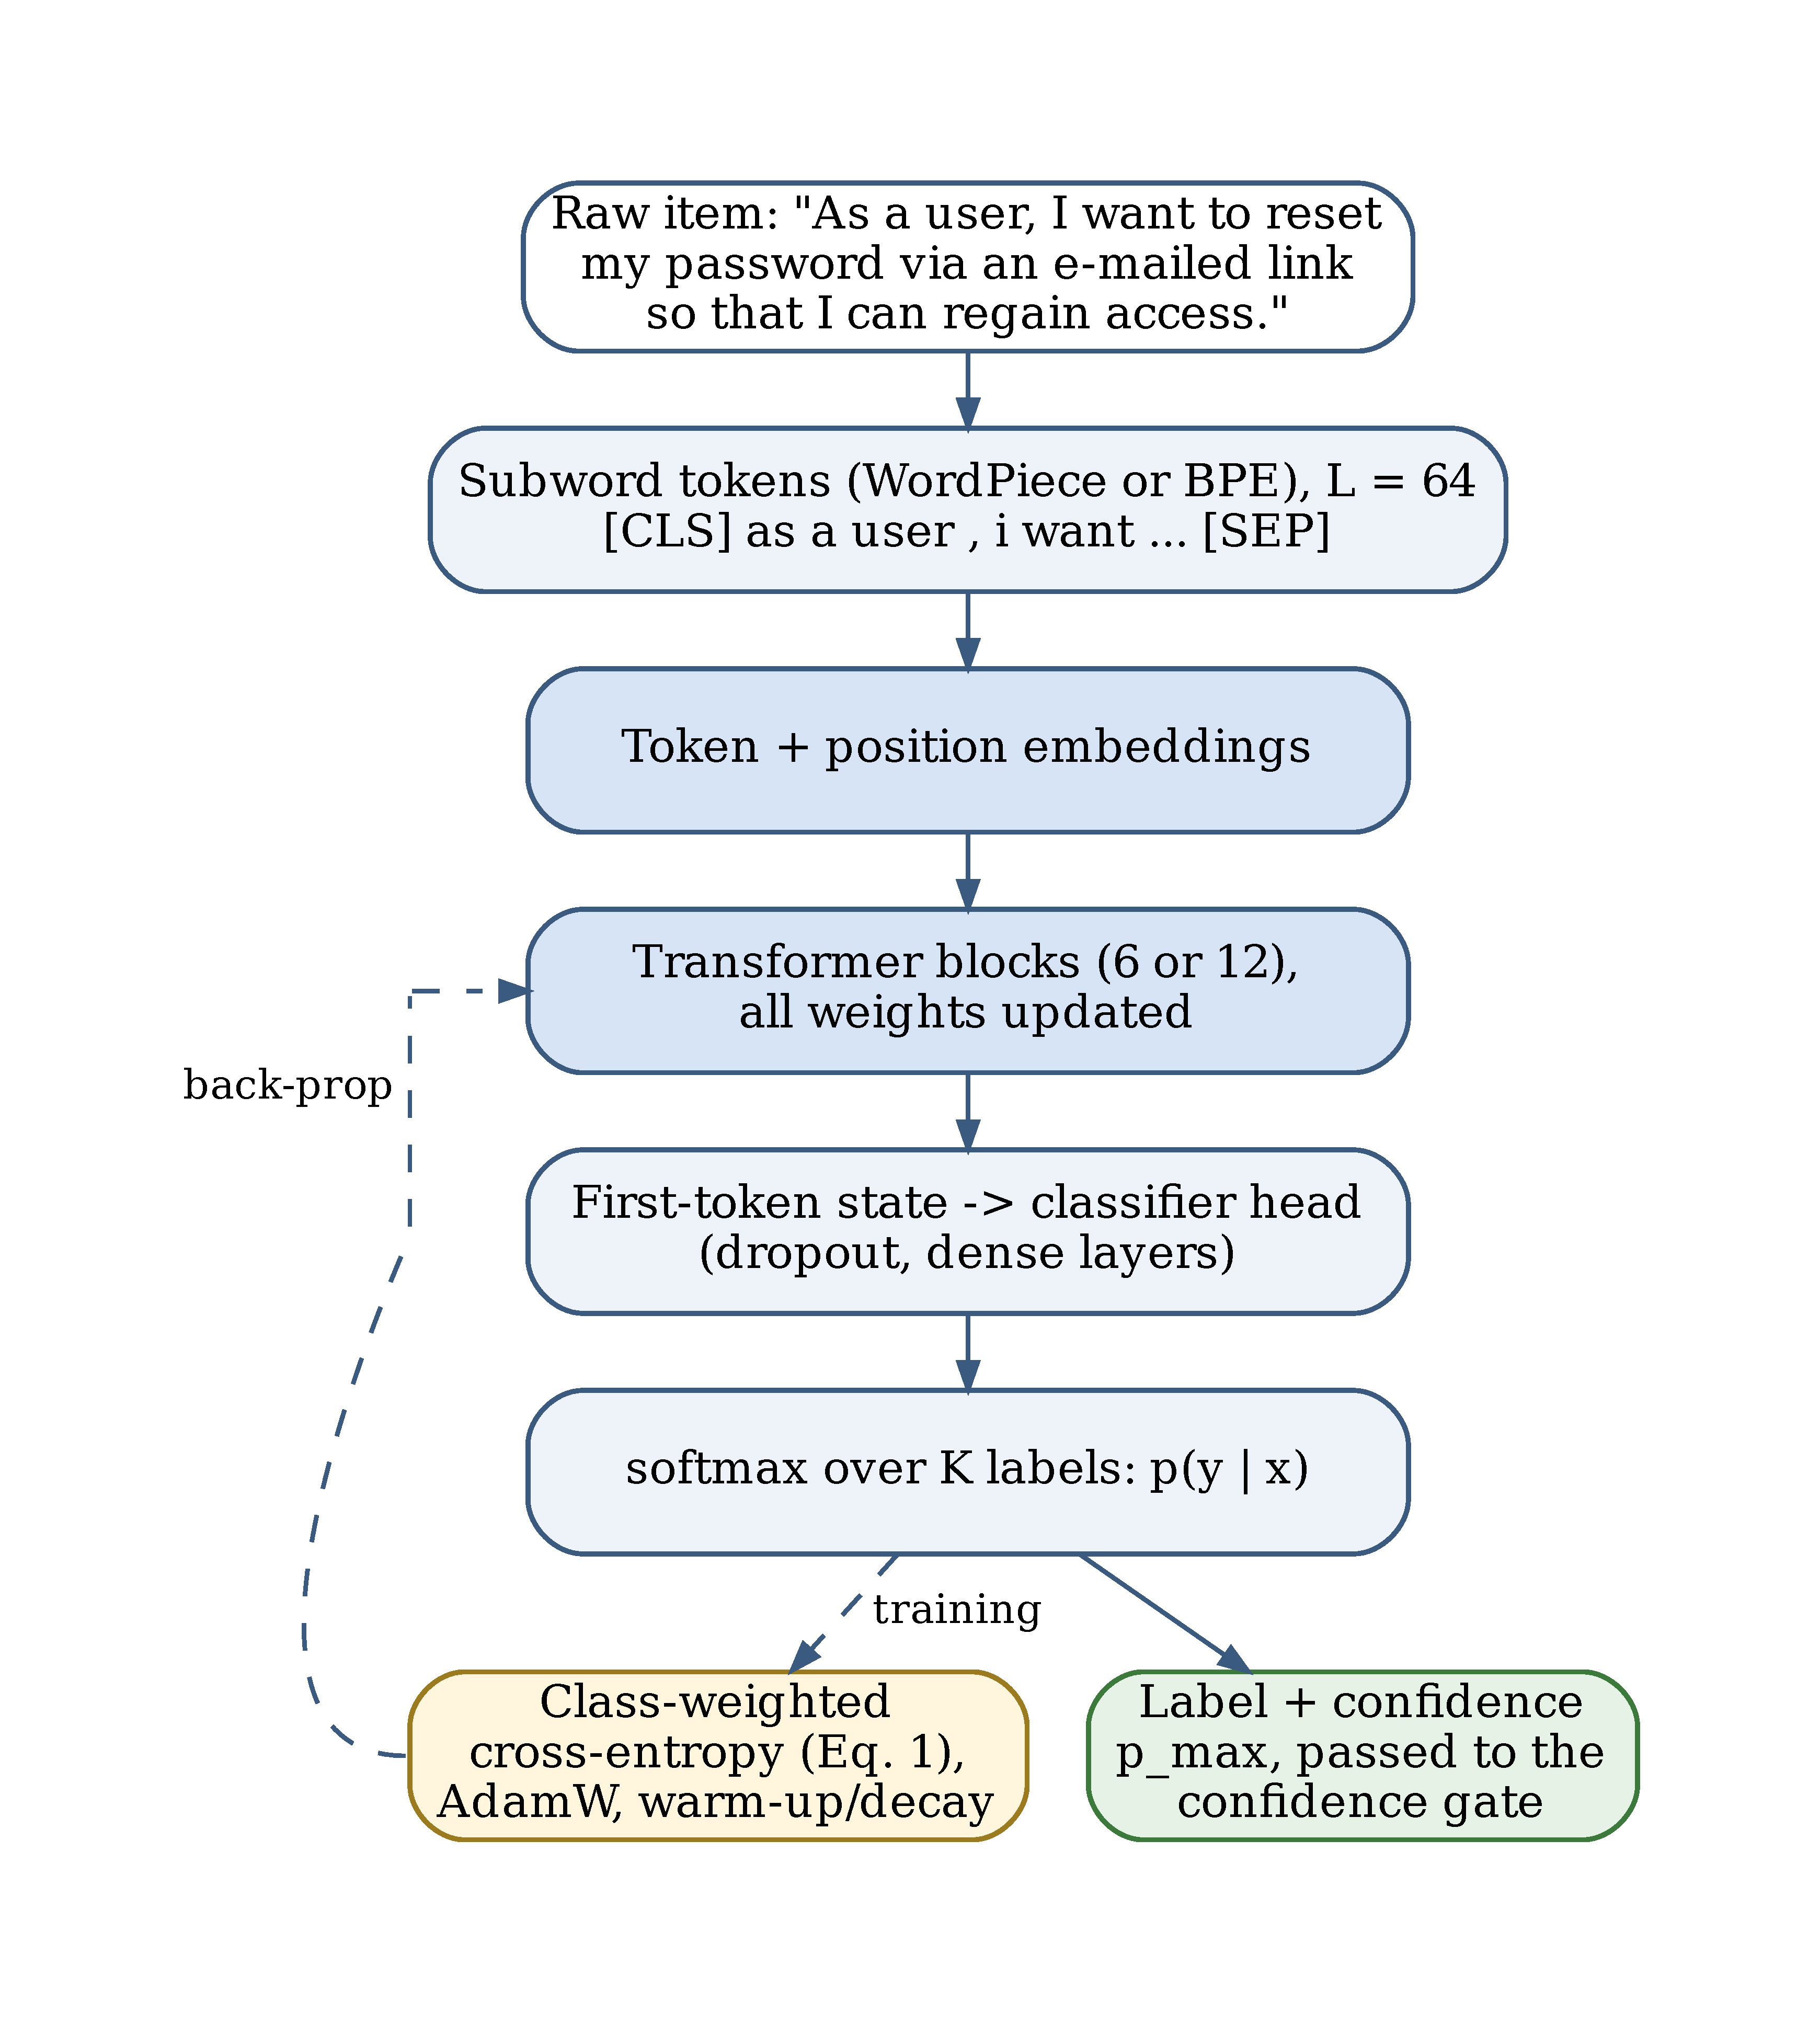
\includegraphics[width=0.94\columnwidth]{fig2_finetune.pdf}
\caption{Fine-tuning pipeline for one backlog item. All weights are updated during fine-tuning; the dashed path is used only during training.}
\label{fig:ft}
\end{figure}

\subsection{Confidence Gate}\label{sec:gate}
A classifier that is wrong 8\% of the time and gives no warning will gradually erode the team's trust in the backlog. The framework therefore applies a label automatically only when the model is confident:

\begin{equation}
\mathrm{route}(x) = \begin{cases} \text{auto-label } \hat{y}, & \max_c p_\theta(c \mid x) \ge \tau \\ \text{Product Owner review}, & \text{otherwise} \end{cases}
\label{eq:gate}
\end{equation}
The threshold $\tau$ in (\ref{eq:gate}) is set on held-out data so that the automatically applied labels reach a precision the team agrees on, for example 0.95. Softmax probabilities from fine-tuned neural networks are often over-confident~\cite{guo2017calibration}, so the framework first rescales them by temperature scaling: the logits are divided by a single constant $T>0$, fitted on held-out items by minimising the negative log-likelihood, before the softmax is taken. This leaves the predicted label unchanged and adjusts only the confidence. Items below the threshold appear in the refinement queue with the two most likely labels shown, which turns a silent error into a one-click decision.

\subsection{Integration with the Backlog Workflow}
Fig.~\ref{fig:flow} places the classifier in the Scrum cycle. When an item is created or edited, the tracker sends it to the service, which writes back a label and a confidence value. During refinement the team reviews the low-confidence queue and also checks the high-confidence quality labels, because these carry consequences. A security label, for instance, adds the team's security checklist to the item's acceptance criteria. A performance label prompts the team to state a measurable target, such as “search results appear within 2 s for 95\% of queries.” Usability items get an accessibility check. Before sprint planning, the Product Owner can filter the ordered backlog by label and see, for example, that the next three sprints contain no operability work. Ordering stays with the Product Owner~\cite{scrumguide2020}; the classifier makes quality work visible but never reorders the backlog.

\begin{figure*}[!t]
\centering
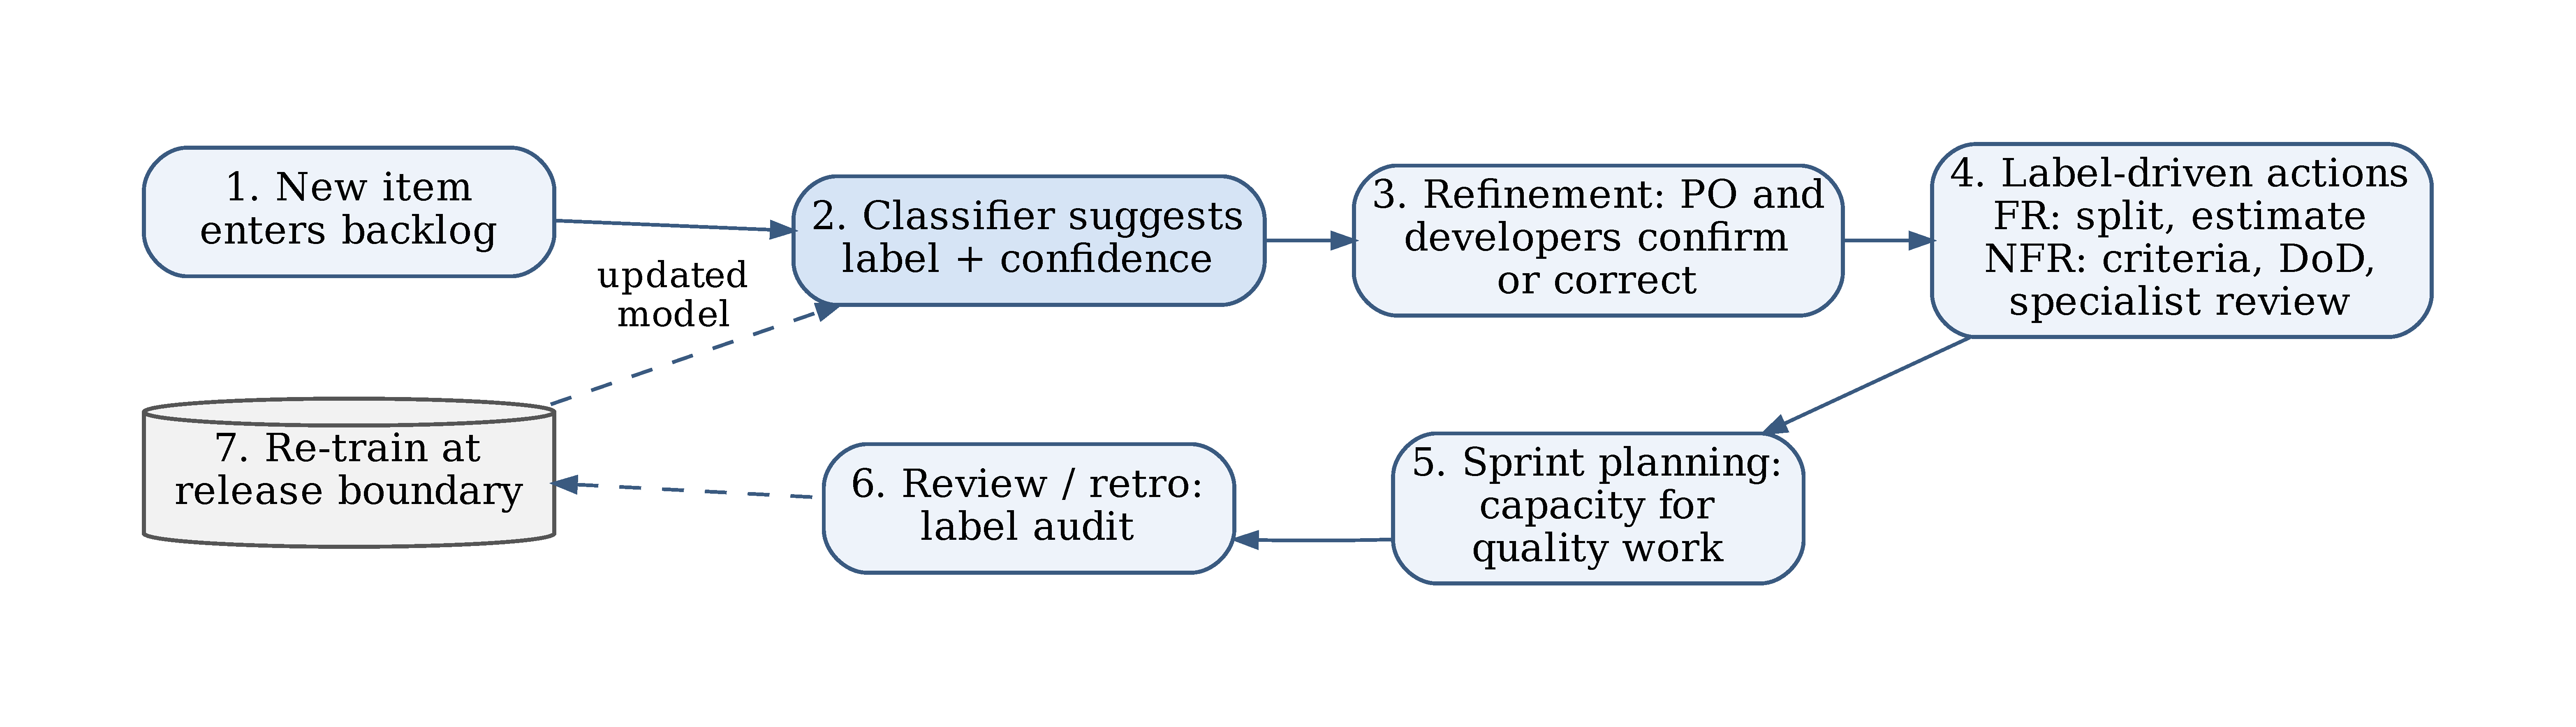
\includegraphics[width=0.99\textwidth]{fig3_workflow.pdf}
\caption{Classifier-in-the-loop backlog workflow. Corrections made during refinement are logged and used for re-training at release boundaries.}
\label{fig:flow}
\end{figure*}

\subsection{Human Feedback and Re-Training}
Every label the Product Owner confirms or changes is stored together with the item text, the model version and the confidence. The model is re-trained at release boundaries rather than continuously, so that its behaviour stays stable within a sprint. Two signals tell the team when re-training is due: the share of items routed to review rising above an agreed level, and the precision of automatic labels, measured on a small random audit sample, falling below the target.

\section{Experimental Setup and Results}\label{sec:exp}
This section has two parts. Section~\ref{sec:ownexp} reports experiments that \emph{we ran ourselves}. Section~\ref{sec:litres} summarises results \emph{reported in the literature}, which we did not reproduce. The two are kept separate throughout, and no literature number appears in our results table.

\subsection{Our Comparative Experiment}\label{sec:ownexp}
\emph{Data.} We used the PROMISE NFR dataset from its Zenodo record~\cite{promisenfr2007}: 625 labelled requirements from 15 projects. Table~\ref{tab:data} gives the class distribution, together with an agile-style example that we wrote for each class to show what the label means in a backlog. The PROMISE items themselves are “shall” statements, not user stories. We defined two tasks. Task A separates functional (255) from non-functional (370) requirements. Task B classifies the four most frequent quality classes: usability (67), security (66), operability (62) and performance (54), 249 items in total. The seven remaining quality classes have between 1 and 38 examples, too few for a reliable per-class estimate, so we left them out.

\begin{table*}[!t]
\centering
\caption{PROMISE NFR class distribution (625 requirements, 15 projects) and illustrative backlog items.}
\label{tab:data}
\footnotesize
\setlength{\tabcolsep}{3pt}
\renewcommand{\arraystretch}{1.12}
\begin{tabular}{>{\raggedright\arraybackslash}p{0.7cm}>{\raggedright\arraybackslash}p{1.9cm}>{\raggedright\arraybackslash}p{0.6cm}>{\raggedright\arraybackslash}p{0.8cm}>{\raggedright\arraybackslash}p{11.2cm}}
\toprule
\textbf{Code} & \textbf{Class} & \textbf{n} & \textbf{Task} & \textbf{Illustrative agile item (written by us, not from PROMISE)} \\
\midrule
F & Functional & 255 & A & “As a user, I want to reset my password via an e-mailed link so that I can regain access.” (F; also carries a security aspect) \\
US & Usability & 67 & A, B & “As a screen-reader user, I want every form field to have a label so that I can complete checkout.” \\
SE & Security & 66 & A, B & “As an administrator, I want failed login attempts logged with time and IP so that I can spot attacks.” (F+SE) \\
O & Operability & 62 & A, B & “As an operator, I want to change the backup schedule without a redeploy.” \\
PE & Performance & 54 & A, B & “As a shopper, I want search results within 2 s so that I do not abandon the search.” \\
LF & Look and feel & 38 & A & “As a marketer, I want pages to use the corporate colour palette.” \\
A & Availability & 21 & A & “As a customer, I want the shop to be reachable 99.9\% of the time.” \\
SC & Scalability & 21 & A & “As the business, we want to serve 10,000 concurrent users at launch.” \\
MN & Maintainability & 17 & A & “As a developer, I want tax rules in configuration rather than in code.” \\
L & Legal & 13 & A & “As a data-protection officer, I want users to be able to export their personal data.” \\
FT & Fault tolerance & 10 & A & “As a user, I want my cart preserved if the payment service fails.” \\
PO & Portability & 1 & A & “As a user, I want the app to run on Android 12 and later.” \\
\bottomrule
\end{tabular}
\end{table*}

\begin{table*}[!t]
\centering
\caption{Our experiments: macro-F1, mean $\pm$ SD over seeds 42–44. PROMISE columns use pooled out-of-fold predictions; random = stratified 10-fold, project = project-held-out 5-fold; Task A: FR vs. NFR (n = 625), Task B: US/SE/O/PE (n = 249). External columns: models trained on all of PROMISE with its original labels or the relabelled quality aspect~\cite{dalpiaz2019}, tested on the 246 external items that have only a functional or only a quality aspect. The SVM is deterministic on the external test, hence SD 0. $^{\ddagger}$ No training; one run over all items, listed under “project” because the model never saw the test project. Best mean per column in bold.}
\label{tab:res}
\footnotesize
\setlength{\tabcolsep}{3pt}
\renewcommand{\arraystretch}{1.12}
\begin{tabular}{@{}lcccccc@{}}
\toprule
\textbf{Model} & \textbf{A random} & \textbf{A project} & \textbf{B random} & \textbf{B project} & \textbf{Ext. original} & \textbf{Ext. relabelled} \\
\midrule
TF-IDF+SVM & 0.912 $\pm$ 0.003 & 0.590 $\pm$ 0.013 & 0.821 $\pm$ 0.015 & 0.718 $\pm$ 0.001 & 0.638 $\pm$ 0.000 & 0.632 $\pm$ 0.000 \\
DistilBERT & 0.909 $\pm$ 0.002 & 0.736 $\pm$ 0.024 & 0.892 $\pm$ 0.016 & \textbf{0.825 $\pm$ 0.022} & 0.708 $\pm$ 0.076 & 0.712 $\pm$ 0.015 \\
BERT-base & 0.915 $\pm$ 0.004 & 0.765 $\pm$ 0.010 & 0.858 $\pm$ 0.004 & 0.774 $\pm$ 0.002 & 0.711 $\pm$ 0.072 & 0.700 $\pm$ 0.005 \\
RoBERTa-base & \textbf{0.917 $\pm$ 0.011} & \textbf{0.806 $\pm$ 0.028} & \textbf{0.913 $\pm$ 0.024} & 0.810 $\pm$ 0.018 & \textbf{0.719 $\pm$ 0.094} & \textbf{0.781 $\pm$ 0.033} \\
Qwen2.5-1.5B, zero-shot$^{\ddagger}$ & – & 0.408 & – & 0.716 & 0.530 & – \\
\bottomrule
\end{tabular}
\end{table*}

\emph{External test data.} To test transfer beyond PROMISE we used the public materials of Dalpiaz et al.~\cite{dalpiaz2019}~\cite{dalpiaz2019data}. They contain requirements from four projects outside PROMISE (Dronology, ReqView, a library system from Leeds, and WASP), annotated with separate functional (F) and quality (Q) aspects, and a relabelled copy of PROMISE with the same two aspects. We dropped the 4 external items that carry neither aspect, leaving 327 items: 96 from Dronology, 84 from Leeds, 86 from ReqView and 61 from WASP. Of these, 187 are only functional, 59 only quality and 81 have both aspects (F+Q). None of the external texts occurs in PROMISE. Like PROMISE, they are specification sentences rather than user stories.

\emph{Protocols.} On PROMISE we used two protocols, and within each one all models share the same splits. \emph{Random}: stratified 10-fold cross-validation (scikit-learn), in which requirements from one project fall on both sides of a split. \emph{Project-held-out}: five folds built with StratifiedGroupKFold using the PROMISE project identifier as the group, so no project contributes to both training and test data. Every model was run with seeds 42, 43 and 44 under both protocols. For each run we pool the out-of-fold predictions and compute per-class precision, recall and F1, their macro averages and accuracy; Table~\ref{tab:res} reports macro-F1 as mean $\pm$ standard deviation over seeds. To compare each transformer with the SVM we used a paired cluster bootstrap: for the pooled predictions of one seed we resampled the 15 projects with replacement 1,000 times, recomputed the difference in macro-F1 each time, and took the 2.5th and 97.5th percentiles as a 95\% interval. Resampling whole projects respects the dependence between requirements written for the same project. For the external test, each model was trained once per seed on all of PROMISE, either with its original labels (F versus NFR) or with the relabelled quality aspect (the 612 relabelled items that carry at least one aspect), and then applied to the external items. The main metric is the macro-F1 for predicting the quality aspect on the 246 items that have only one aspect; we also report precision, recall and F1 of the quality flag on all 327 items. Differences from the SVM were tested with a paired bootstrap that resamples items within each document (2,000 resamples), with the difference averaged over the three seeds. We did no hyper-parameter search for any model. Tuning on the same folds would have made the comparison look better without making it more honest. Code, splits and every model's predictions are in our reproducibility package.

\begin{figure*}[!t]
\centering
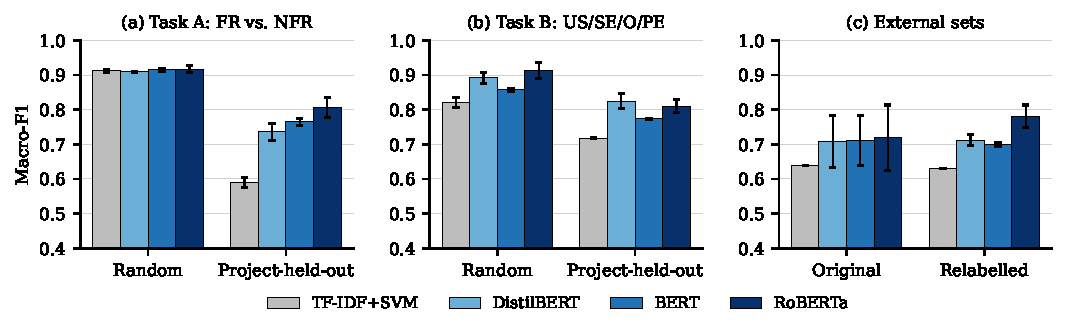
\includegraphics[width=1.00\textwidth]{fig4_results.pdf}
\caption{Our experiments: macro-F1, mean over seeds 42–44 with SD error bars, under random 10-fold and project-held-out 5-fold splits of PROMISE NFR and on the external industrial requirements (trained on all of PROMISE with original or relabelled labels). The y-axis starts at 0.4.}
\label{fig:res}
\end{figure*}

\emph{Models.} The baseline uses TF-IDF features over word unigrams and bigrams, with sublinear term frequency and English stop-word removal, fitted inside each training fold, and a linear SVM (C = 1, class-balanced weights). We fully fine-tuned three encoders with the Hugging Face Transformers library, with all weights trainable: distilbert-base-uncased~\cite{sanh2019distilbert}, bert-base-uncased~\cite{devlin2019} and roberta-base~\cite{liu2019roberta}. Settings: maximum length 64 tokens (the median item has 21–22 tokens, depending on the tokeniser, and 6–9 of the 625 items were truncated), batch size 16, AdamW with learning rate 5$\times 10^{-5}$ for DistilBERT and 3$\times 10^{-5}$ for BERT and RoBERTa, weight decay 0.01, 10\% linear warm-up followed by linear decay, gradient clipping at 1.0, five epochs, and the class-weighted loss of (\ref{eq:wce}). The models were trained on Google Colab GPU runtimes; the log of the external-test runs records an NVIDIA A100, while the PROMISE runs did not record the GPU type. As a reference that needs no training, we also prompted Qwen2.5-1.5B-Instruct~\cite{qwen2024} zero-shot. For each task one prompt listed the classes with a one-line definition each, and the predicted class was the option letter with the highest next-token probability.

\emph{Calibration.} We measured the expected calibration error (ECE) with 15 equal-width confidence bins. Both the temperature of Section~\ref{sec:gate} and the threshold $\tau$ of (\ref{eq:gate}) were cross-fitted: for each test fold they were fitted only on the out-of-fold predictions of the other folds. $\tau$ was the smallest value on a grid from 0.50 to 0.995 (step 0.005) at which at least 20 items reached a precision of 0.95. For the external test, the temperature and $\tau$ were fitted on the Task A project-held-out predictions of the same model and seed and then applied unchanged.

\emph{Results.} Table~\ref{tab:res} and Fig.~\ref{fig:res} give the macro-F1 results. \emph{Random folds.} On Task A the four models are statistically tied: their mean macro-F1 ranges from 0.909 to 0.917, and none of the nine project-bootstrap intervals for a transformer minus the SVM excludes zero. On Task B the transformers pull ahead. RoBERTa reaches 0.913 $\pm$ 0.024 and DistilBERT 0.892 $\pm$ 0.016, against 0.821 $\pm$ 0.015 for the SVM; their intervals exclude zero in three and two of three seeds respectively. BERT (0.858 $\pm$ 0.004) is ahead of the SVM on average, but none of its intervals excludes zero.

\emph{Project-held-out folds.} Holding out whole projects lowers every score (right-hand columns of Table~\ref{tab:res} and Fig.~\ref{fig:res}), but not equally. On Task A the SVM loses 32 points of macro-F1 and ends at 0.590 $\pm$ 0.013, whereas the transformers lose 11–17 points: DistilBERT reaches 0.736 $\pm$ 0.024, BERT 0.765 $\pm$ 0.010 and RoBERTa 0.806 $\pm$ 0.028. Eight of the nine project-bootstrap intervals exclude zero; the exception is DistilBERT with seed 42 (difference 0.108, 95\% interval $-$0.029 to 0.229). Most of the loss is in the functional class. Averaged over seeds, functional recall falls to 0.27 for the SVM, 0.53 for DistilBERT, 0.56 for BERT and 0.67 for RoBERTa, while non-functional recall stays at 0.93 or above for every model. On an unseen project the models therefore label many functional requirements as non-functional; even the best model finds only about two thirds of them. A likely but untested reason is that functional requirements are written in each project's domain vocabulary, whereas quality requirements reuse phrases such as “shall be available” or “within 2 seconds” across projects. Task B loses less: the SVM drops to 0.718 $\pm$ 0.001, DistilBERT reaches 0.825 $\pm$ 0.022 and RoBERTa 0.810 $\pm$ 0.018, and both are ahead of the SVM in every seed. BERT (0.774 $\pm$ 0.002) is again ahead on average without any interval excluding zero. The drop should not be read as the effect of unseen projects alone, because the protocols differ in other ways. Five project-held-out folds train on about 80\% of the items, against 90\% for ten random folds (on Task A, 409–600 training items per fold instead of about 562). The folds are also uneven, because PROMISE projects differ in size and content: Task A test folds hold between 25 and 216 items, and projects 11–15 contain no functional requirements at all.

\emph{Calibration and the confidence gate.} The raw softmax scores were over-confident on unseen projects. On Task A project-held-out folds the expected calibration error (ECE) of the three transformers was 0.16–0.19, and a threshold of 0.95 on the raw scores would have auto-labelled 82\%–91\% of the items at a precision of only 0.81–0.85. BERT was badly calibrated on Task B as well (ECE 0.27–0.30, against 0.11 or less for DistilBERT and RoBERTa). Cross-fitted temperature scaling reduced the Task A project-held-out ECE to 0.04–0.05, but it also showed how little of that task can be automated safely: after scaling, no Task A item of an unseen project reached a confidence of 0.95, and the cross-fitted threshold auto-labelled at most 22\% of the items (RoBERTa), at a precision of 0.82, short of the 0.95 target. Task B behaved better. With the cross-fitted threshold, DistilBERT auto-labelled 53\% of the unseen-project items at a precision of 0.95, RoBERTa 65\% at 0.93 and BERT 30\% at 0.91; the remaining items would go to review. Under random folds the same procedure auto-labelled about 88\% of Task A items at a precision of 0.95, which again shows how optimistic random splits are.

\emph{External test.} Trained on all of PROMISE with its original labels and applied to the 327 industrial requirements, the SVM reached a macro-F1 of 0.638 on the 246 items that have only a functional or only a quality aspect. The transformers reached 0.708 $\pm$ 0.076 (DistilBERT), 0.711 $\pm$ 0.072 (BERT) and 0.719 $\pm$ 0.094 (RoBERTa), and the within-document bootstrap put their seed-averaged advantage over the SVM at +0.070 to +0.081, with every interval excluding zero. The large standard deviations come mostly from seed 44, which gave 0.612–0.628 for all three transformers against 0.722–0.790 for seeds 42 and 43. Training on the relabelled PROMISE instead changed little for the SVM, DistilBERT and BERT (all intervals for the difference include zero), but it raised RoBERTa to 0.781 $\pm$ 0.033, a gain of 0.062 (95\% interval 0.030 to 0.093). As a quality flag over all 327 items, every model reached an F1 between 0.67 and 0.71. The errors differ, however: with the original labels the transformers flagged 33\%–34\% of the purely functional items as having a quality aspect, against 45\% for the SVM, and flagged 59\%–60\% of the mixed F+Q items. Results also varied by document. RoBERTa reached 0.78 on Leeds and 0.78 on ReqView, but only 0.45 on Dronology and 0.40 on WASP, where only 2 and 6 items are purely quality requirements, so those two values rest on very few items. The calibration did not transfer well. With the temperature fitted on the PROMISE out-of-fold predictions of the same model and seed, the external ECE fell from 0.16–0.35 to 0.07–0.23, so the scores stayed miscalibrated. A threshold for 0.95 precision could be set on PROMISE in eight of the nine runs. Applied unchanged to the external items, it auto-labelled 12\%–44\% of them (30–109 items) at a precision of 0.82–1.00, and met the target in only 5 of the 8 runs; the three failures were the seed-44 runs of all three transformers.

\emph{Zero-shot LLM.} Without any training, Qwen2.5-1.5B-Instruct reached a macro-F1 of 0.408 on Task A, because it called only 8\% of the requirements non-functional although 59\% are. On Task B it reached 0.716, about the same as the SVM on unseen projects. On the external items it flagged only 4\% of the items with a quality aspect (macro-F1 0.530). A model of this size with one fixed prompt is a weak baseline, and larger models or few-shot prompts may do much better; we did not test them.

Our untested reading of the contrast between the tasks is this. In PROMISE the FR/NFR split under random folds is carried largely by surface cues, such as verbs of action versus adjectives of quality, and a bag of n-grams captures these well. Telling usability from operability or security is harder: words such as “user”, “system” and “shall” appear in every class, and each class has only 54–67 examples. This is the situation in which pre-trained representations are expected to help most. Some errors also support the F+Q view of Dalpiaz et al.~\cite{dalpiaz2019}. One requirement states that all changes to a dispute case be “recorded in the case history”; PROMISE labels it non-functional (legal), yet all three transformers called it functional in every random-fold run, and it reads like the audit-log example in Table~\ref{tab:data}. A requirement to conform to the Americans with Disabilities Act is labelled usability, but RoBERTa predicted security in all six of its Task B runs, and arguably it is a legal requirement as well. Fold-level accuracy also varied widely (DistilBERT, seed 42, random Task B folds: 0.80 to 0.96 over test folds of about 25 items), which is why we report pooled scores.

\subsection{Reported Results from the Literature}\label{sec:litres}
Table~\ref{tab:lit} lists the results reported in the literature. These are the authors' numbers, not ours. On PROMISE NFR the published results bracket our own. For the FR/NFR decision, NoRBERT reports an F1 of up to 94\%~\cite{hey2020norbert} and Eltahier et al. report 0.99~\cite{eltahier2025}, both above our random-fold macro-F1 of 0.909–0.917 for the three transformers. For the frequent quality classes, our random-fold RoBERTa reaches 0.913, higher than the 87\% average F1 that NoRBERT reports. We do not read this as RoBERTa beating NoRBERT. The protocols and metrics differ: we used random stratified folds over four classes and report macro-F1, and our own project-held-out runs in Table~\ref{tab:res} score well below our random-fold runs, although that gap also reflects smaller training sets. NoRBERT's corrected report also lowers its unseen-project improvement from 15 to 10 percentage points~\cite{hey2022corrected}, another sign that headline numbers depend on the split. Model size also differs: NoRBERT fine-tuned BERT base and large models, whereas all our encoders are base-size or smaller. Our random-fold TF-IDF+SVM macro-F1 of 0.912 on Task A is close to the roughly 92\% precision and recall reported by Kurtanović and Maalej~\cite{kurtanovic2017} and to the F-measure of 0.91 that Dias Canedo and Cordeiro Mendes~\cite{diascanedo2020} report for TF-IDF models on the larger PROMISE\_exp, so the classical baseline appears to be reasonably reproduced. The 0.99 reported by Eltahier et al. is a weighted F1 with hyper-parameters chosen by ablation on the same data, so it cannot be placed on the same protocol as our untuned macro-F1. Finally, Dalpiaz et al.~\cite{dalpiaz2019} evaluated their own classifiers on the external documents we used; we did not reproduce their setup, so we do not set our numbers beside theirs.

\section{Discussion}\label{sec:disc}
\subsection{What the Evidence Supports}
Taken together, the sources support three claims and leave a fourth open. First, fine-tuned transformers are at least as good as feature-engineered models on PROMISE-style text and are better at transferring to unseen projects~\cite{hey2020norbert,hey2022corrected}. Second, the FR/NFR boundary is not crisp: an item can carry both aspects~\cite{dalpiaz2019}, and backlog items mix several requirements in one entry~\cite{vancan2025}. Third, label-free approaches are possible but still well behind supervised ones~\cite{alhoshan2023,luo2022prcbert}. Our own results sharpen this picture. Under random folds a linear TF-IDF model was as good as any transformer for the coarse FR/NFR decision, whereas RoBERTa and DistilBERT were clearly better at separating quality classes. Moving to project-held-out folds cost the SVM 32 points of macro-F1 on Task A but the transformers only 11–17, part of which may come from smaller training sets and uneven test folds rather than from unseen projects alone. The transformers' advantage is therefore largest where it matters for adoption, on projects they have not seen, which agrees with the unseen-project results of NoRBERT~\cite{hey2020norbert,hey2022corrected}. The external test points the same way, with a smaller margin: on documents written by other teams and labelled by other researchers, the transformers stayed ahead of the SVM, but their scores (0.708–0.719) were far below the random-fold numbers and varied strongly with the seed and the document. Two cautions follow. BERT-base, the original model of the family, was the weakest transformer on Task B and the worst calibrated, so the choice of encoder matters even within one family. And calibration is not portable: temperature scaling fixed most of the miscalibration on held-out PROMISE folds, but a threshold chosen on PROMISE missed its precision target on the external documents in 3 of 8 runs. For a team, the practical consequence is that any model, and especially its confidence threshold, should be re-checked on the team's own items before its labels are trusted. The open question is how well any of these models works on genuine backlog text, where items are terse, informal and full of project jargon.

\subsection{Implications for Backlog Management}
For a Scrum team the value lies less in the label itself than in the conversation it starts. Picture a team refining twenty new stories before sprint planning. The classifier tags fourteen with high confidence. It flags “As an administrator, I want to see a log of all login attempts” as functional with a security concern, and it sends three ambiguous items to the review queue. The Product Owner confirms the security tag, so the team adds retention and access rules to the acceptance criteria before the work starts, not after a later audit. Used this way, the classifier supports the Definition of Done and leaves responsibility for ordering and scope with the Product Owner~\cite{scrumguide2020}. It also complements story-quality checks such as QUS~\cite{lucassen2016qus}: one tool asks whether a story is well formed, the other asks what kind of concern it raises.

\subsection{Challenges}
Table~\ref{tab:chal} summarises the main deployment challenges and how the framework addresses each one. Three need further comment. \emph{Imbalance} is structural: some quality classes will always be rare, and accuracy can mislead on imbalanced data~\cite{johnson2019}, which is why we report macro-averaged scores. \emph{Format shift} is the largest unknown: models trained on “The system shall…” sentences meet “As a $\langle$role$\rangle$…” stories, bug reports and one-line chores in a real tracker~\cite{vancan2025}. \emph{Label drift} follows from the backlog being an informal and evolving model of the work~\cite{sedano2019}: a team's notion of “operability” may change as its product matures.

\begin{table}[!t]
\centering
\caption{Deployment challenges, supporting evidence and mitigations.}
\label{tab:chal}
\scriptsize
\setlength{\tabcolsep}{3pt}
\renewcommand{\arraystretch}{1.12}
\begin{tabular}{>{\raggedright\arraybackslash}p{2.35cm}>{\raggedright\arraybackslash}p{2.0cm}>{\raggedright\arraybackslash}p{3.2cm}}
\toprule
\textbf{Challenge} & \textbf{Evidence} & \textbf{Mitigation in the framework} \\
\midrule
Class imbalance (PO: 1 item; FT: 10) & \cite{johnson2019} & Weighted loss (Eq. 1); macro-F1; merge rare classes \\
FR/NFR ambiguity, mixed items & \cite{dalpiaz2019,vancan2025} & F+Q label; split multi-requirement items \\
SRS-to-story format shift & \cite{lucassen2016use,vancan2025} & Parse role/goal/benefit; fine-tune on team data \\
Over-confident predictions & \cite{guo2017calibration}; our Section~\ref{sec:ownexp} & Temperature scaling; re-set threshold on team data; audit sample \\
Optimistic random splits & \cite{hey2022corrected}; our Section~\ref{sec:ownexp} & Project-held-out or time-based evaluation before roll-out \\
Scarce labelled data & \cite{alhoshan2023,tunstall2022setfit} & Zero-/few-shot start; active labelling in review \\
Compute and privacy limits & \cite{sanh2019distilbert} & Distilled model on-premise; no external API \\
\bottomrule
\end{tabular}
\end{table}

\subsection{Threats to Validity}\label{sec:threats}
\emph{Construct validity.} PROMISE labels were assigned by students around 2007~\cite{clelandhuang2007}, and the FR/NFR boundary itself is contested~\cite{dalpiaz2019}. A model that agrees with these labels has learned one annotation convention, not a ground truth; the external labels follow another group's convention. \emph{Internal validity.} We used three seeds, no hyper-parameter search and common default learning rates. A different configuration could change the rankings where the bootstrap intervals include zero, notably BERT on Task B and the random-fold tie on Task A. GPU training is not bit-for-bit reproducible, so a rerun may give slightly different numbers; for that reason the reproducibility package stores every model's predictions. The SVM and the transformers did share identical folds. \emph{External validity.} Random 10-fold splits put requirements from the same project into both training and test data. Our project-held-out runs show how much lower the scores are when this is prevented, but the gap is not a pure measure of that leakage: the project-held-out models also train on less data (about 80\% of the items instead of 90\%), and their test folds differ in size and class mix, with projects 11–15 contributing no functional requirements. The external test adds four documents, but only 246 items enter its main metric, and Dronology and WASP contain very few purely quality requirements. All these texts are English specification sentences, so our results say nothing direct about user stories or other languages. We did try to build a user-story test set: two annotators labelled 242 user stories as functional, non-functional or both, but their agreement was at chance level (Cohen's $\kappa$ = $-$0.002), so the labels cannot serve as ground truth and we report no story-level results. \emph{Conclusion validity.} With 15 projects, the cluster bootstrap resamples few units and its intervals are coarse. The external results varied strongly with the seed (seed 44 was the weakest for every transformer), and three seeds give only a rough estimate of that spread. The zero-shot baseline used one small model and one prompt, and PROMISE may be part of its pre-training data. Finally, the literature synthesis is not a systematic review, and relevant studies may have been missed.

\subsection{Ethical and Practical Considerations}
Backlogs can contain customer names, contract details and security weaknesses. Sending them to an external API may breach confidentiality, which is a practical argument for small models that run on-premise. Automation bias is the other risk: if a high-confidence label is never questioned, the team may stop thinking about quality at all. Keeping the label visible but editable, and auditing a sample every release, limits that risk.

\section{Conclusion and Future Work}\label{sec:concl}
We set out to judge whether BERT-family classifiers can support agile backlog management. The literature shows steady progress on PROMISE-style text, from indicator terms to NoRBERT, but also a habit of reporting near-ceiling scores under protocols that cannot be compared. Our own comparative experiments found that on random folds the fully fine-tuned DistilBERT, BERT and RoBERTa were no better than a linear SVM at separating functional from non-functional requirements (macro-F1 0.909–0.917), but RoBERTa and DistilBERT were clearly better at telling the four most frequent quality classes apart. When whole projects were held out, every model lost ground, and the first task changed from a statistical tie to a clear transformer lead (0.736–0.806 against 0.590). On 327 industrial requirements from four other projects the transformers kept a smaller lead over the SVM, and its bootstrap intervals excluded zero. Even so, the best model found only about two thirds of the functional requirements of an unseen project, and confidence thresholds did not carry over from PROMISE to new documents, so a confidence gate needs calibration on the team's own items before it can be trusted. We therefore propose using such models as refinement assistants: they surface quality concerns early and route uncertain items to a person, while ordering and scope remain with the Product Owner.

Four steps would make the evidence stronger. (1) Build an openly licensed corpus of real user stories and backlog items with F/Q aspect labels, written labelling guidelines and measured inter-annotator agreement; our own pilot annotation did not reach usable agreement. (2) Make project-held-out and time-ordered splits the standard; our runs cover 19 projects in total and no time order. (3) Compare fine-tuned encoders with larger instruction-tuned models, few-shot prompting and SetFit under one protocol, using label budgets a real team could afford. (4) Run a field study in which a team uses the confidence-gated classifier during refinement, recalibrated on its own items, and measure whether quality issues are found earlier.

\section*{Acknowledgment}
The author thanks Shairy Kalra, Lovely Professional University, for supervising this work.

\bibliographystyle{IEEEtran}
\bibliography{references}
\end{document}